\documentclass[main.tex]{subfiles}


\begin{document}

\chapter{Introduction}
This doctoral thesis presents a collection of topics that are relevant
in decision making under uncertainty, primarily motivated by
problems in the retail industry.
We will speak primarily about the decision process involved in setting the
price of products, including demand modelling, estimation from data,
handling of uncertainty, and optimization algorithms.

The process of pricing products in order to control demand and
maximize revenues has been undertaken for centuries. In recent
decades, data- and model-driven approaches have become increasingly
popular in order to advise on and automate the process for companies.
There are several success stories from early adopters, for example in
the airline industry.
American Airlines estimated in 1992 that the introduction of revenue
management software had, over the preceding three
years, contributed \SI{500}[\$] million of additional revenue per year,
and would continue to do so in the future~\cite{smith1992yield}.
In an example from Chilean retail, the authors of~\cite{bitran1998coordinating}
report an expected revenue improvement of \SIrange{7}{16}{\percent} after implementing
model-driven strategies.
This range of financial impact due to implementation of pricing and revenue
management systems are further supported in other studies, see \cite[Ch.~1.2]{phillips2005pricing}.
For retailers with billions of pounds in revenues, small
improvements to their revenue-management processes can be worth millions
of pounds.
In addition unsold items add up to thousands of tonnes of waste per year, so
improving the control of demand for products is advantageous
for both retailers and the environment.

The theory and practice of pricing and revenue management is highly
multi-disciplinary, and attracts research from a wide variety of
fields. Our focus will be on different aspects of the modelling and
optimization procedures, from a more mathematical point of view.
\citet{phillips2005pricing} and \citet{ozer2012oxford} contain perspectives on the
revenue management process prevalent in the social sciences.
A notable resource with more mathematical focus, which
cover both theoretical and practical
perspectives, is that of those of \citet{talluri2006theory}.
Other approaches to pricing of retail products more akin to the
mathematical modelling community can, for example, be found in~\cite{butler2014customer}.
\todo[inline]{Mention proprietary knowledge, cite talluri}

\section{Outline of the thesis}
\textbf{TODO:} Just use the stuff in ``Making decisions'' below?

\section{Making decisions}
The approach to decision making considered in this thesis consists of
five general steps, of which each chapter will touch on a subset.
The steps are summarised as follows.
\begin{enumerate}
\item Objective --- statement of what the decision maker wants to achieve.
\item Model of the system --- mathematical modelling of relevant aspects
  needed to achieve the objective.
\item Data assimilation --- incorporation of available observations in
  the mathematical model.
\item Risk preference --- mathematical modelling of the decision maker's risk
  preference.
\item Optimization --- algorithms and approximations required to
  evaluate different decisions.
\end{enumerate}
\todo[inline]{TiKZ diagram from Trinity talk?}
In \Cref{ch:onestage} we focus on the general discussion of the
Objective, Risk preferences, and Optimization.
Following that, \Cref{ch:discrete_control} and
\Cref{ch:cts_control} discuss  aspects of the steps Model of the system, Risk
preferences, and Optimization.
These three chapters are closely linked to the application of pricing
in retail, whilst the remaining chapters have a mathematical focus
independent of particular application.
\Cref{ch:koopestim} looks at a novel way to handle the Data
assimilation step. Finally, \Cref{ch:objaccel} presents a new
algorithm to improve the Optimization step.\todo{Paragraph necessary?}

The objectives we focus on in this thesis are aspects
of sales, revenue, and profit targets that can be influenced by
pricing decisions.\todo{Move to section?}
At the core of such decisions lies models connecting price and demand of products.
In \Cref{sec:intro_model_demand} we summarise the classic approaches
to demand modelling in revenue management, for reference in later
chapters.
The demand models often include unobservable parameters that are
inferred from data.
These models are used to forecast future demand, sometimes months in
the future.
The uncertainty of future events, and estimates of model
parameters, will be described as random variables within a probability
theoretical framework. \Cref{sec:intro_prob_rvs} covers preliminary
theory of probability, random variables and stochastic
processes.\todo{Move to section?}

\section{Modelling demand}\label{sec:intro_model_demand}
We define demand as the quantity of a product that people are willing
to buy per time period, at a particular price. For the purpose of our
work, demand may change over time, even if the price is constant.
Time-dependent aspects of demand include periodic effects, such as
seasonality and longer term trends.
In addition to pricing decisions, retailers can use advertisements and
offers to improve sales. Such demand control mechanisms often have a
more significant impact on sales than price changes in their own
right. They are harder to forecast accurately, however, and will not
be considered further in this thesis.

The relationship between price and demand are often described in a
continuum fashion, rather than at discrete levels such as pounds or
pence. We are interested in retailers with large-scale sales and
aggregate demand models where treating the demand as a continuum gives
a reasonable approximation.
In both academia and industry, simple demand curves often used to
model the price-demand relationship of
products. See~\cite[Ch.~7.3]{talluri2006theory} or~\cite{phillips2005pricing}
for a discussion of the most popular demand curves. They are often
chosen in order to simplify the parameter
estimation procedure, in practice, or simplify the analysis, for academic purposes.

We denote the demand for a given product at price $a\geq 0$, holding
other aspects such as time and competitor product prices constant, by $q(a)$.
This thesis will make use of a range of demand curves, in particular
\begin{align}\label{eq:demand_fun_lin}
  q(a) &= q^{(1)}-q^{(2)}a,&q^{(1)},q^{(2)}&>0,&\text{linear demand}&,\\
  q(a) &= e^{q^{(1)}-q^{(2)}a},&q^{(1)}\in\mathbb{R},q^{(2)}&>0,&\text{exponential
                                                                  demand}&\text{, and}\\
  q(a) &= q^{(1)}a^{-q^{(2)}},&q^{(1)},q^{(2)}&>0,&\text{power demand}&.\label{eq:demand_fun_pow}
\end{align}
Note that these functions can only be considered as local
approximations to demand. That is, we use these models to predict
aggregate demand responses in a neighborhood of the current
price. Care must especially be taken if one is to use the power demand
function: The demand goes to infinity as price goes to zero, and
revenues go to infinity as price goes to infinity for products with $q^{(2)}\in(0,1)$.
\Cref{fig:demandfun_comparison} provides a comparison of the three
demand curves, and shows that they behave very similarly close to the
current price, $a=1$.
\begin{figure}[htbp]
  \centering
  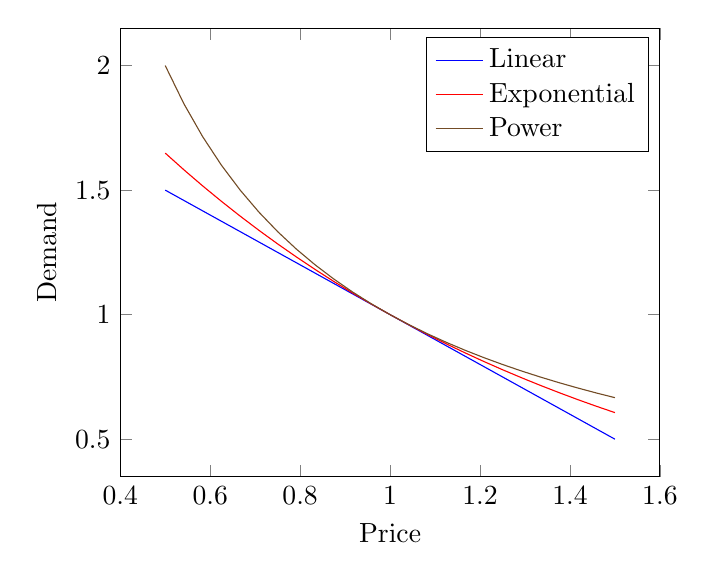
\begin{tikzpicture}[baseline]
    \begin{axis}[
      xlabel={Price},
      ylabel={Demand},
      legend cell align=left,
      ]
      \addplot+[domain=0.5:1.5, mark=none] {2-x};
      \addlegendentry{Linear}
      \addplot+[domain=0.5:1.5, mark=none] {exp(1-x)};
      \addlegendentry{Exponential}
      \addplot+[domain=0.5:1.5, mark=none] {1/x};
      \addlegendentry{Power}
    \end{axis}
  \end{tikzpicture}
  \caption{Comparison of demand curves. The units of price and time
    have been re-scaled so that $q(1)=1$.}\label{fig:demandfun_comparison}
\end{figure}

In cases where we believe that the price of one product affects the
demand of another product, we introduce cross-effects on the demand
functions. For products $j=1,2,\dots,J$, denote their respective prices by
$a=(a_1,a_2,\dots,a_J)$, and their demands by $q_j(a)$.
One way to extend the demand curves in~\eqref{eq:demand_fun_lin}
to~\eqref{eq:demand_fun_pow} to a multi-product case is, according to \cite{talluri2006theory},
\begin{align}
  q_j(a)&=q_{j}^{(1)}-\sum_{l=1}^Jq_{j,l}^{(2)}a_l,
  &\text{linear demand}&,\\
  q_j(a)&=\exp\left( q_{j}^{(1)}-\sum_{l=1}^Jq_{j,l}^{(2)}a_l
          \right),
  &\text{exponential demand}&\text{, and}\\
  q_j(a)&=q_j^{(1)}\prod_{l=1}^Ja_l^{-q_{j,l}^{(2)}},
  &\text{power demand}&.
\end{align}
The valid domains of the parameters vary. For example, a linear demand
model where we believe that increasing the price of product $l$ has a
positive effect on the demand of product $j$ constrains
$q_{j,l}^{(2)}$ to be negative. \Cref{fig:demand_exponential_two}
provides an example of demand for a given product when varying the
its price and the price of one competing product, using the exponential demand function.

\todo[inline]{Introduce my model, if we need it in chapter on
  one-stage}
\begin{figure}[htbp]
  \centering
  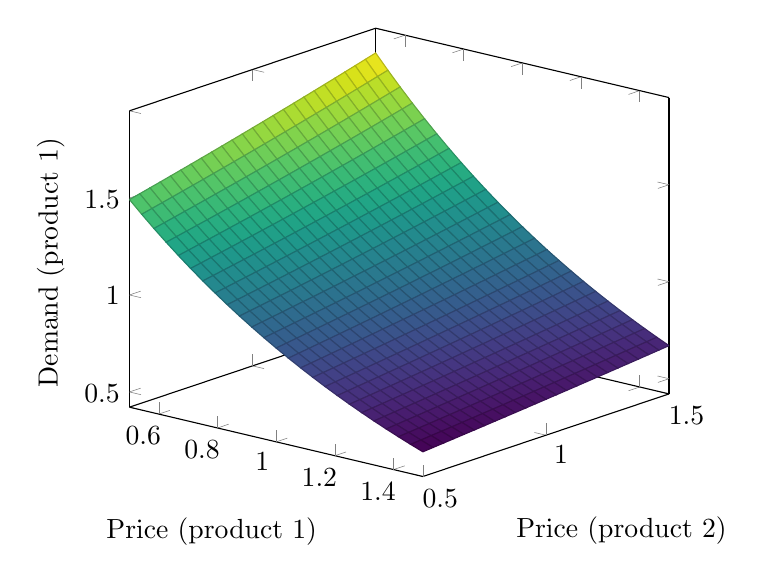
\begin{tikzpicture}
    \begin{axis}[
      domain=0.5:1.5,
      xlabel={Price (product 1)},
      ylabel={Price (product 2)},
      zlabel={Demand (product 1)},
      view={40}{20},
      colormap/viridis
      ]
      \addplot3[surf]
      {exp(1-0.2-1*x+0.2*y)};
    \end{axis}
  \end{tikzpicture}
  \caption{Exponential demand function for product $1$, with one
    competing product $j=2$.
    Units are rescaled so that $q_1(\vecbracks{1,1})=1$.
  }\label{fig:demand_exponential_two}
\end{figure}

\subsection{Forecasting and uncertainty}
Demand models, such as those presented above, have parameters that are
product specific, and which must be estimated before forecasts of
demand can be made.
As multi-month forecasts may be required by the retailer, better
approximations to future demand are likely achieved with
time-dependencies in the parameters.
This estimation procedure is often guided by
historic sales data collected by the retailer, using data assimilation
techniques~\cite{law2015data} and time series analysis~\cite{chatfield2004analysis}.
\todo[inline]{Provide example of time-dependent modelling? 1)
  Sinusoidal model, 2) Model based on neighbouring values, linear
  combination of previous time periods (in a periodic domain,
  i.e. both the most recent, and in previous years/months)}

The models used in forecasting future demand at particular prices carry
a range of errors and uncertainty. First, estimates of parameter values are not
exact. Second, the model form may be
inappropriate. Third, exogenous events impact demand outcomes in a more general
way.
% These sources of uncertainty are all epistemic, meaning
% that one can reduce them by refining models and gathering more
% data.
% Fourth, uncertainties that are aleatory, which refers to inherent
% uncertainty in a system that cannot be reduced. See
% \cite{der2009aleatory} for a discussion on aleatory and epistemic
% uncertainty.
% One may argue the philosophical point whether uncertainty that is
% aleatory exists, however, it does not change our approach to modelling
% the uncertainty in our forecasts.
A forecast is in essence an extrapolation of a validated model to a
region of the input domain not yet experienced. We may still have an
idea of what form the uncertainty of this extrapolation takes, which
in this thesis will be described in terms of random variables.

For example, consider a product for which we forecast the sales for
two consecutive periods using the exponential demand model,
\begin{equation}
  q(t,a) =
  e^{q^{(1)}(t)-q^{(2)}(t)a},\qquad t=1,2.
\end{equation}
To quantify the uncertainty in our model parameters, we associate
each of $q^{(1)}(t)$, $q^{(2)}(t)$ a probability distribution, not
necessarily independent.
Let $W(t,a)$ denote a random field that expresses the uncertainty
associated with extrapolating outside the observed price region, as
well as exogenous events.
We forecast the demand in period $t$ to be $Q(t,a)=q(t,a)W(t,a)$, and
the total forecasted demand is thus the random variable $Q(1,a_1) +
Q(2,a_2)$, where $a_t$ denotes the planned price in period $t$.

\section{Decisions via optimisation}\label{sec:intro_decisions_through_optim}
Optimisation is central to our approach to decision making, and will
be integral to all the chapters in the thesis.
We will cover optimisation in the context of multiple objectives,
one-stage decision problems, sequential decision problems, parameter
estimation, and in algorithm design.
All the problems we consider will eventually confirm to a general
form. For some decision set $\mathcal{X}$, and a mapping
$\mathcal{F}:\mathcal{X}\to\mathbb{R}$ that is bounded below, we
formulate the decision problem as finding a solution to
\begin{equation}
  \min_{x\in\mathcal{X}}\mathcal{F}(x).
\end{equation}
The set $\mathcal{X}$ may be a subset of a finite or
infinite-dimensional space. Whenever the problem needs to be solved by
a numerical approach, we discretise the set and consider
finite-dimensional approximations $X\subset\mathbb{R}^n$, $f:X\to\mathbb{R}$ to
$\mathcal{X}$ and $\mathcal{F}$ respectively.
The set $X$ can be defined either implicitly, or explicitly, in the
form of a collection of equality and inequality constraints,
\begin{equation}
  X = \{x\in\mathbb{R}^n\mid c_i(x)=0, c_k(x)\geq 0, \text{ for }
  i\in\mathcal{I},\;j\in\mathcal{J}\}.
\end{equation}
\todo[inline]{Minimize vs maximise}
\todo[inline]{Local minima}
The theory of optimisation of functions on $\mathbb{R}^n$, and
algorithms to approximate solutions to such problems, are well covered
by~\citet{nocedal2006numerical}. We will often refer to this book in
the context of optimisation.

\section{Preliminary probability and random variables}\label{sec:intro_prob_rvs}
\todo[inline]{Do we need this?}

\biblio{} % Bibliography when standalone
\end{document}

%%% Local Variables:
%%% mode: latex
%%% TeX-master: t
%%% TeX-command-extra-options: "--shell-escape"
%%% End:
